\chapter{Risultati preliminari}
\section{Dataset}
Nella prima versione sviluppata, il dataset di immagini generate utilizzando PIL è illustrato nelle immagini \ref{fig:out}

\begin{figure}[!h]
  \centering
  \begin{minipage}[b]{0.5\textwidth}
    \tcbox[boxsep=0mm, boxrule=0.5mm, 
            colframe=black!30!black, colback=white]
            {
\includegraphics[width=\textwidth]{pictures/g1.png}}
    % \caption{}
    \label{}
  \end{minipage}
  \begin{minipage}[b]{0.5\textwidth}
    \tcbox[boxsep=0mm, boxrule=0.5mm, 
            colframe=black!30!black, colback=white]
            {
\includegraphics[width=\textwidth]{pictures/g2.png}}
    % \caption{}
    \label{}
  \end{minipage}\\
  \begin{minipage}[b]{0.5\textwidth}
    \tcbox[boxsep=0mm, boxrule=0.5mm, 
            colframe=black!30!black, colback=white]
            {
\includegraphics[width=\textwidth]{pictures/g3.png}}
    % \caption{}
    \label{}
  \end{minipage}
  \begin{minipage}[b]{0.5\textwidth}
    \tcbox[boxsep=0mm, boxrule=0.5mm, 
            colframe=black!30!black, colback=white]
            {
\includegraphics[width=\textwidth]{pictures/g4.png}}
    \caption{In figura sono mostrati 4 esempi di immagini realizzate secondo i criteri illustrati}
    \label{fig:out}
  \end{minipage}
\end{figure}
Le immagini utilizzate come dataset nella prima versione sono semplici immagini 400 x 40 x 1 in cui ho considerato un singolo dominio internet (e.g Google, Facebook, Apple, ...) generando, nel mio caso, 1024 immagini contenenti quel dominio e utilizzando questo set di immagini come Dataset (come input della DCGAN)\\
In una seconda versione ho incluso nelle immagini del dataset, una maschera di rumore per riprodurre un dataset più dinamico e far in modo che il modello generasse caratteri imprecisi (che è proprio il mio scopo). Nella figura \ref{fig:ou2} è possibile notare la densità del rumore (non ho scelto una densità troppo alta, in quanto il modello non risultava convergere).
\begin{figure}[!h]
  \centering
  \begin{minipage}[b]{0.5\textwidth}
    \tcbox[boxsep=0mm, boxrule=0.5mm, 
            colframe=black!30!black, colback=white]
            {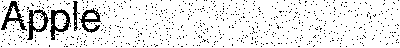
\includegraphics[width=\textwidth]{pictures/a1.png}}
    % \caption{}
    \label{}
  \end{minipage}
  \begin{minipage}[b]{0.5\textwidth}
    \tcbox[boxsep=0mm, boxrule=0.5mm, 
            colframe=black!30!black, colback=white]
            {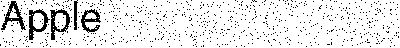
\includegraphics[width=\textwidth]{pictures/a2.png}}
    % \caption{}
    \label{}
  \end{minipage}\\
  \begin{minipage}[b]{0.5\textwidth}
    \tcbox[boxsep=0mm, boxrule=0.5mm, 
            colframe=black!30!black, colback=white]
            {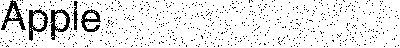
\includegraphics[width=\textwidth]{pictures/a3.png}}
    % \caption{}
    \label{}
  \end{minipage}
  \begin{minipage}[b]{0.5\textwidth}
    \tcbox[boxsep=0mm, boxrule=0.5mm, 
            colframe=black!30!black, colback=white]
            {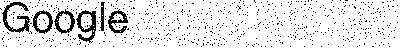
\includegraphics[width=\textwidth]{pictures/gg1.png}}
    \caption{La seconda versione del dataset utilizzato dalla DCGAN per produrre immagini. Da notare il rumore aggiunto}
    \label{fig:ou2}
  \end{minipage}
\end{figure}\\
%%%%%%%%%%%%%%%%%%%%%
Una versione più avanzata del modello sarebbe quella di generare immagini aventi padding arbitrario come mostrato in figura \ref{fig:out3}.
\begin{figure}[!h]
  \centering
  \begin{minipage}[b]{0.5\textwidth}
    \tcbox[boxsep=0mm, boxrule=0.5mm, 
            colframe=black!30!black, colback=white]
            {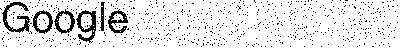
\includegraphics[width=\textwidth]{pictures/gg1.png}}
    % \caption{}
    \label{}
  \end{minipage}
  \begin{minipage}[b]{0.5\textwidth}
    \tcbox[boxsep=0mm, boxrule=0.5mm, 
            colframe=black!30!black, colback=white]
            {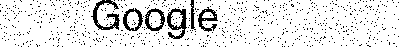
\includegraphics[width=\textwidth]{pictures/gg2.png}}
    % \caption{}
    \label{}
  \end{minipage}\\
  \begin{minipage}[b]{0.5\textwidth}
    \tcbox[boxsep=0mm, boxrule=0.5mm, 
            colframe=black!30!black, colback=white]
            {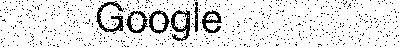
\includegraphics[width=\textwidth]{pictures/gg3.png}}
    % \caption{}
    \label{}
  \end{minipage}
  \begin{minipage}[b]{0.5\textwidth}
    \tcbox[boxsep=0mm, boxrule=0.5mm, 
            colframe=black!30!black, colback=white]
            {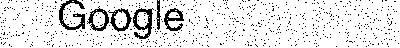
\includegraphics[width=\textwidth]{pictures/gg4.png}}
    \caption{Questa versione del dataset presenta padding randomico su entrambi gli assi.}
    \label{fig:out3}
  \end{minipage}
\end{figure}\\
Infine, un'ultima challenge sarebbe quella di produrre un modello che sia in grado di generare immagini, da un dataset di ingresso che utilizza più font, come quelli mostrati in figura \ref{fig:out4}
\begin{figure}[!h]
  \centering
  \begin{minipage}[b]{0.5\textwidth}
    \tcbox[boxsep=0mm, boxrule=0.5mm, 
            colframe=black!30!black, colback=white]
            {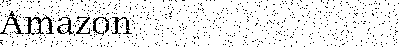
\includegraphics[width=\textwidth]{pictures/am1.png}}
    % \caption{}
    \label{}
  \end{minipage}
  \begin{minipage}[b]{0.5\textwidth}
    \tcbox[boxsep=0mm, boxrule=0.5mm, 
            colframe=black!30!black, colback=white]
            {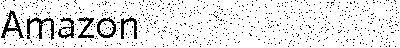
\includegraphics[width=\textwidth]{pictures/am2.png}}
    % \caption{}
    \label{}
  \end{minipage}\\
  \begin{minipage}[b]{0.5\textwidth}
    \tcbox[boxsep=0mm, boxrule=0.5mm, 
            colframe=black!30!black, colback=white]
            {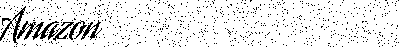
\includegraphics[width=\textwidth]{pictures/am3.png}}
    % \caption{}
    \label{}
  \end{minipage}
  \begin{minipage}[b]{0.5\textwidth}
    \tcbox[boxsep=0mm, boxrule=0.5mm, 
            colframe=black!30!black, colback=white]
            {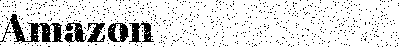
\includegraphics[width=\textwidth]{pictures/am4.png}}
    \caption{Questo dataset presenta immagini con domini scritti utilizzando font differenti.}
    \label{fig:out4}
  \end{minipage}
\end{figure}
\section{Dati generati}
Una volta prodotto il dataset, ho utilizzato la DCGAN per analizzare le immagini che era in grado di produrre, cercando di lavorare sui vari strati convoluzione/deconvoluzione in modo da renderla il più fedele possibile.\\
Dalla prima versione del dataset [\ref{fig:out}], il modello non è riuscito a produrre immagini che rappresentassero in maniera corretta i domini squatted, il problema risiedeva nel fatto che il dataset di partenza era troppo statico (le immagini erano completamente identiche l'une dalle altre). Questo non ha permesso alla rete di produrre immagini con sufficiente rumore tra le singole lettere. In figura \ref{fig:v1} è visualizzato l'output del modello nella versione 1, mentre in figura \ref{fig:lossesv1} un estratto della losses dopo 1000 epoch.
\begin{figure}[!h]
  \centering
  \begin{minipage}[b]{\textwidth}
    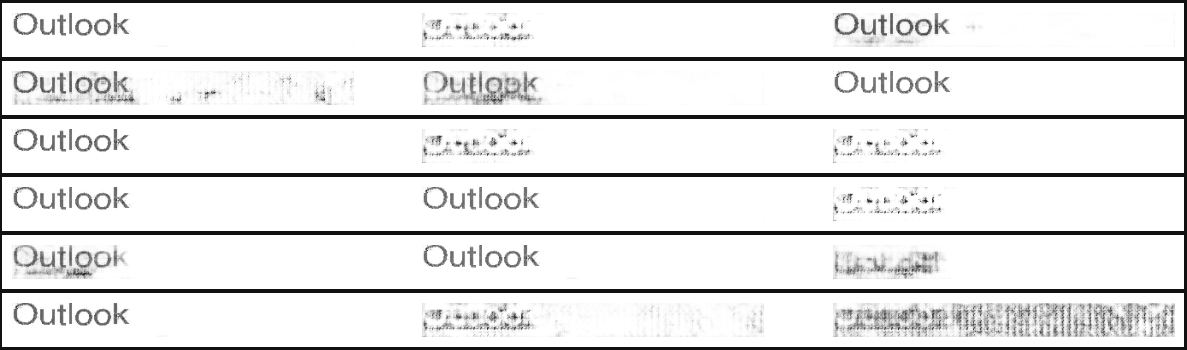
\includegraphics[width=\textwidth]{pictures/picsv1.png}
    \caption{I risultati del modello nella prima versione del dataset}
    \label{fig:v1}
  \end{minipage}
  \hfill
\end{figure}

\begin{figure}[!h]
  \centering
  \begin{minipage}[b]{0.9\textwidth}
    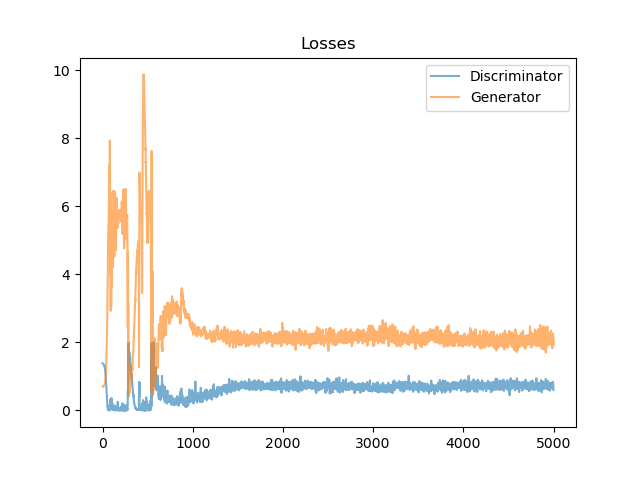
\includegraphics[width=\textwidth]{pictures/lossesV1.png}
    \caption{losses nella versione 1. Da notare che il generatore ha una loss abbastanza alta rispetto al discriminatore}
    \label{fig:lossesv1}
  \end{minipage}
  \hfill
\end{figure}
Nella seconda versione, avendo immagini con rumore casuale all'interno del dataset, la rete converge in maniera più corretta verso le immagini reali producendo anche testo avente lettere distorte dal rumore (che è proprio quello che si vuole produrre). In figura \ref{fig:dcganv2} un esempio di output per la seconda versione del modello. In figura \ref{fig:lossesv2} l'andamento delle losses nell'arco di 1000 epoche.
\begin{figure}[!h]
  \centering
  \begin{minipage}[b]{\textwidth}
    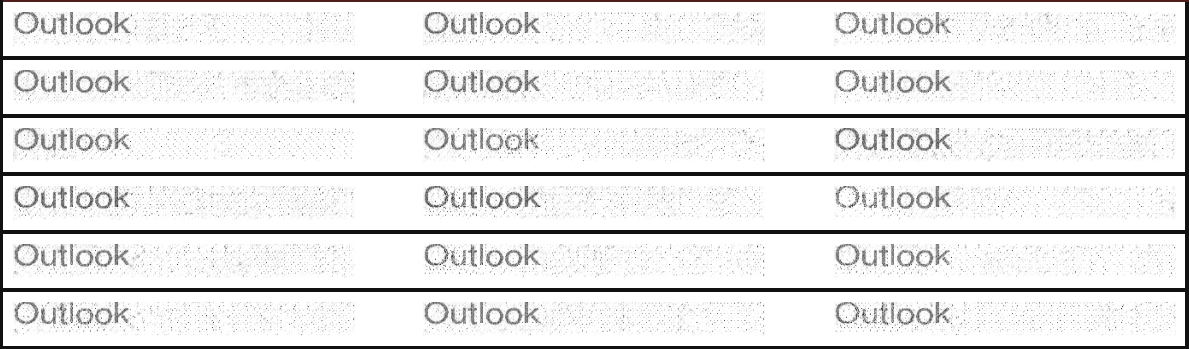
\includegraphics[width=\textwidth]{pictures/maxpool.png}
    \caption{Output della DCGAN nella seconda versione. Il test è stato effettuato sul dominio "Outlook". Questi sono i risultati dopo 1000 epoche.}
    \label{fig:dcganv2}
  \end{minipage}
  \hfill
\end{figure}

\begin{figure}
  \centering
  \begin{minipage}[b]{0.7\textwidth}
  \tcbox[boxsep=0mm, boxrule=0.4mm, 
            colframe=black!10!black, colback=white]
            {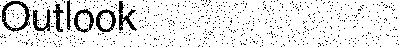
\includegraphics[width=\textwidth]{pictures/staticv1.png}}
    \label{fig:git1}
  \end{minipage}
  \begin{minipage}[b]{0.7\textwidth}
    \tcbox[boxsep=0mm, boxrule=0.4mm, 
            colframe=black!10!black, colback=white]{
            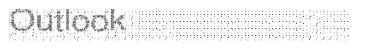
\includegraphics[width=\textwidth]{pictures/singlev1.png}}
    \caption{Immagine prodotta dalla DCGAN dopo 1000 epoche rispetto ad un'immagine del dataset di partenza}
    \label{fig:singlev1}
  \end{minipage}
\end{figure}

\begin{figure}[!htb]
  \centering
  \begin{minipage}[b]{\textwidth}
    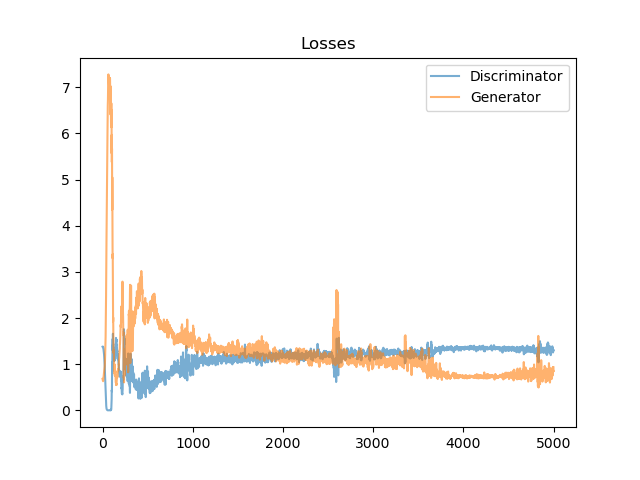
\includegraphics[width=\textwidth]{pictures/loss_maxpool.png}
    \caption{losses utilizzando la seconda versione del dataset. In questa versione la losses è nettamente più decente rispetto alla prima versione.}
    \label{fig:lossesv2}
  \end{minipage}
  \hfill
\end{figure}
Ho anche provato ad usare dei layer di AveragePooling anzichè MaxPooling ma le immagini generate (figura \ref{fig:avgpool}) si presentano molto più sfocate, come previsto.
\begin{figure}[!h]
  \centering
  \begin{minipage}[b]{\textwidth}
    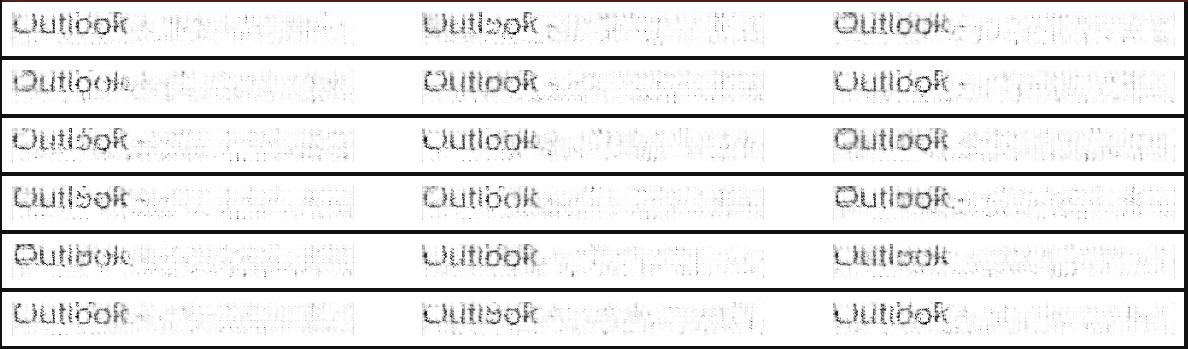
\includegraphics[width=\textwidth]{pictures/avgpool.png}
    \caption{DCGAN nella versione 2. Le immagini generate utilizzando layers di AvgPool al posto di MaxPooling le quali presentano troppe sgranature}
    \label{fig:avgpool}
  \end{minipage}
  \hfill
\end{figure}\\

\section{Validazione}
Utilizzando keras come OCR sono riuscito a produrre delle stringhe di testo partendo dalle immagini in output della rete neurale. Nella prima versione del dataset, non si è riusciti ad estrarre una quantità di domini rilevanti, in quanto le immagini prodotte [\ref{fig:v1}] risultavano appunto prive di rumore e imprecisioni sui caratteri.\\
Per estrarre i potenziali domini di squatting, ho allenato il modello inizialmente con la prima versione del dataset [\ref{fig:v1}] fino a 1000 epoche di addestramento (per le successive versioni del dataset ho utilizzato lo stesso approcio). Successivamente ho fatto produrre alla rete delle immagini di test che ho utilizzato come input per il modulo OCR (Keras). Il modulo OCR produceva una quantità di domini non rilevante e soprattutto con ripetizioni. Ho utilizzato un algorimo per la rimozione dei duplicati ma risultavano essere comunque rilevanti. Il problema non era il fatto che fossero tanti ma che alcuni domini riconosciuti si discostavano troppo da quello che era il dominio di partenza. Per ovviare a questo problema ho utilizzato un algoritmo di Edit Distance (The Levenshtein distance algorithm) per estrarre solo i domini che si discostassero di una certa edit distance dal dominio di partenza. Inzialmente utilizzando come valore di limite 5, ma infine come valore ottimale ho osservato che andasse bene 3.
Qui una lista di potenziali domini di squatting estratti dal Modulo OCR utilizzando la prima versione de dataset.

\begin{verbatim}
outlook,outlock,outlogk,cutlock,outosk,cutgo,cutlook,outlgok,cutlgok,
cutloss,outloock,utogks,wlook,outlouk,outrok.

apple,acoli,pplet,applet,aple,updle,spple,apute,narlle,aprle,appiet,applel,
cpple
\end{verbatim}

Utilizzando invece la seconda versione del dataset, introducendo il rumore alle immagini, si è visto un aumento dei potenziali domini prodotti. Qui una lista per i domini più famosi.

\begin{verbatim}
gutlook,cltlook,cutlook,cutook,dutlook,butlook,butook,gatlook,
cutiook,sutook,sutlook,outlook,sutiook,dutloor,gutook,cutloo,sltlook,
eatlook,eutlook,outiook,duatlook,cutloek,gutloek,cuttook,dutook,suatlook,
outook,dutiook,eutiook,outlooks,autloor,mutlook,suttook,dutlock,oatiook,
oltlook,utook,outtook,sutlock,sutlookk,wutlook,buttook,dutloon,butiook,
cutleok,sutloek,atlook,gutloon,wetlook,gltlook,gutiook,outlooke,outioon,
outloor,cutloor,ontiook,catlook,guatlook,mutook,guttook,putloor,utlook,
cuatlook,gutlock,butlock,oatlook,cutloos,euttook,outlock,sutloor,cutloon,
nutlook,butloak,putloo,duttook,dutloo,bltlook,sutloo,oltook,outloo,dltlook,
butloo,eutlooks,sutloon,eutloor,cutlock,datlook,gutloor,satlook,eutook,
otlook,qutlook,outoek,dutloek,oltlooks,putlook,outlolt,rutlook,olatlook,
dutloos,qutook.

poogle,googe,soogle,google,coogle,gooale,cooge,foogle,saogle,eoogle,gocgle,
oogle,ooge,sooge,cooglle,cooale,cgogle,fooge,gtogle,socgle,goegle,eooge,
ggogle,ooogle,sooale,gdogle,oegle,scogle,sgogle,oocgle,googie,gcogle,saoogle,
sooole,cogle,gogle,fcogle,caoogle,fgogle,fogle,soegle,soosle,sogle,agogle,
googlle,tsoogle.

appias,apdle,saole,faple,appled,adple,sepple,asple,appls,spple,aoples,
eliple,apple,spples,adpls,sltle,appie,apople,aople,atple,acpie,spps,afple,
sapple,fappis,sppie,aple,fapple,applg,faaple,appile,fappie,fadple,ooe,aepie,
applc,aples,aoe,appies,appec,anple,aaple,adplu,sadple,aeals,sadole,adte,
apoles,seple,appe,adols,asol,apples,apole,sadpie,sols,dple,adpole,fapole,
sole,apols,adole,adpe,adpile,acpln,acqie,appla,acole,apile,arple.

amazon,anazon,atazon,aazon,amazan,amnazon,asenazon,aanazon,amezon,
aeazon,eazoc,aaazor,asmazoe,aaazon,aetazon,aazor,armazon,amelzon,amaaon,
amaizon,aeton,ameion,aazos,aaezon,ametzan,amaon,amzon,mazon,amason,
aiazon,amaizan,amtton,amtazon,ameizon,arnazon,amezan,atmazen,ameszon,
rmazon,aanezon,aegazon,aatazon,atazen,amezen,smazon,samazon,aesazon,
aseazon,araen,asmazon,agazon,dazon,amazn,aeaon,orazo,pazon,aezon,amazo,atmazon,
aenazon,anaon,famazon,aazoe,aoazon,anatzon,asnazon,aareon,amaton,auazon,
amazen,anoazon,aazan,ahazon,aaazod,aniizon,aagazos,aeazan,anezon,aagazoen,
ramaizon,amazoe,amaor,annazon,amrzon,
\end{verbatim}


